\documentclass[12pt]{article}

\usepackage[margin=1in]{geometry} % 1-inch margins
\usepackage{times}                % Times (Times New Roman–like) font
\usepackage{fancyhdr}             % For custom headers/footers
\usepackage{graphicx}             % For including images
\usepackage{titlesec}             % For section formatting
\usepackage{amsmath}              % For numbering control
\usepackage{caption}
\usepackage{setspace}             % For line spacing

\pagestyle{fancy}
\fancyhf{} % Clear default header and footer

% Header on the right side
\fancyhead[R]{Saksham AI: Multilingual Virtual Interviewer}

% Footer on the left side
\fancyfoot[L]{Pillai HOC College of Engineering \& Technology (Autonomous), Rasayani}
\fancyfoot[R]{\thepage}

% Horizontal lines in header & footer
\renewcommand{\headrulewidth}{0.4pt} 
\renewcommand{\footrulewidth}{0.4pt} 

% Enable figure numbering at section level (e.g., Figure 8.1, 8.2, 8.3)
\numberwithin{figure}{section}

% Paragraph Formatting
\setlength{\parindent}{1.5em}
\setlength{\parskip}{0em}

\begin{document}

\setcounter{page}{40}

\vspace*{\fill}

\begin{center}
    {\Large \bf Chapter 8} \\[1em]
    {\Large \bf Result Analysis}
\end{center}
\vspace*{\fill}

\newpage

% SECTION 8: RESULT ANALYSIS
\setcounter{section}{8}
\subsection{Result Analysis}

\begin{figure}[h]
\subsubsection*{8.1.1 : User Interface} 
\vspace{20pt}

\begin{center}
\fbox{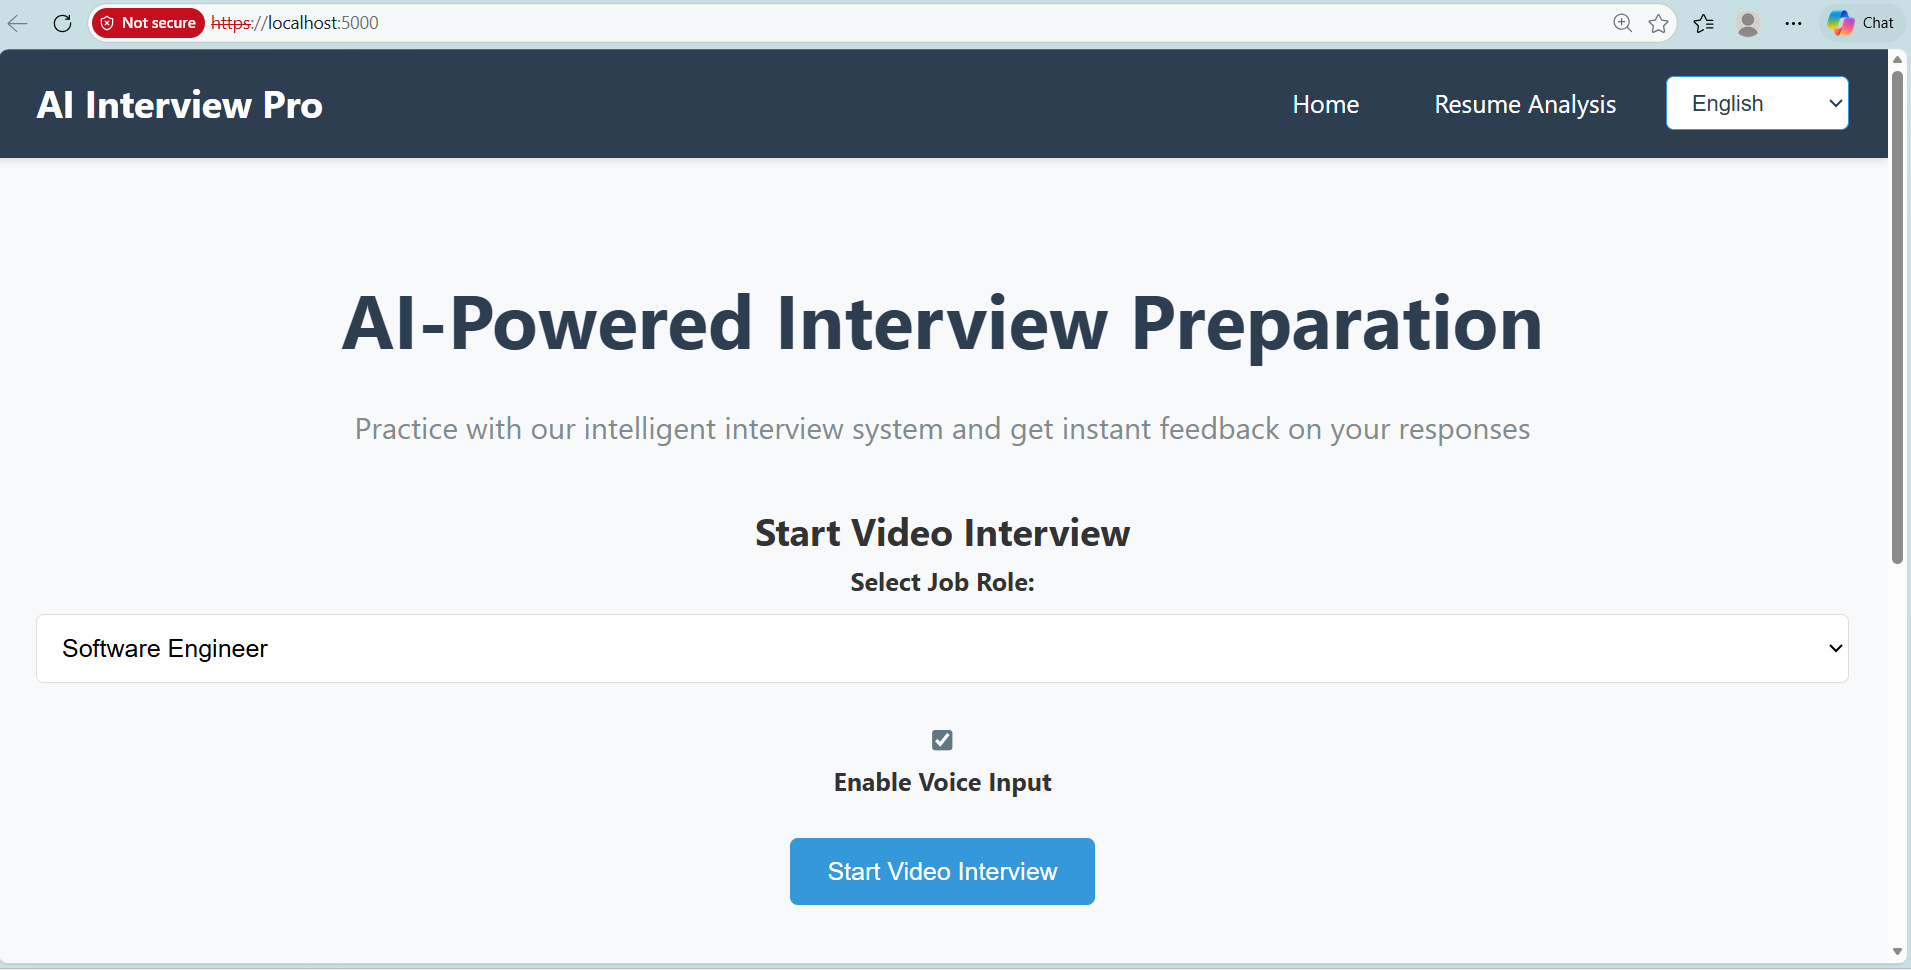
\includegraphics[width=0.99\textwidth]{op_1.png}}
\captionsetup{labelformat=empty}
\caption{Fig 8.1.1: User Interface}
\end{center}

\end{figure}

\vspace{10pt}

\begin{spacing}{1.5}
\noindent The interview initiation interface depicted in  figure 8.1.1 requires candidates to configure their session settings before beginning the practice interview. This interface collects essential preferences, including the target job role, preferred interaction language, and input method. Upon accessing the “Start Video Interview” section, the system prompts the candidate to select a specific job role, such as Software Engineer, from a dropdown menu. For a more realistic and conversational experience, the candidate may enable the “Enable Voice Input” option, which activates the microphone and allows the system to capture spoken responses instead of relying solely on text input. After confirming the selected role, preferred language (via the top navigation bar), and input settings, clicking the “Start Video Interview” button initiates the interactive session. The system then launches the live interview environment, enabling the candidate to practice answering questions and receive immediate feedback on their performance.
\end{spacing}

\newpage

\begin{figure}[h]

\subsubsection*{8.1.2 : Resume Analysis} 

\vspace{10pt}

\begin{center}
\fbox{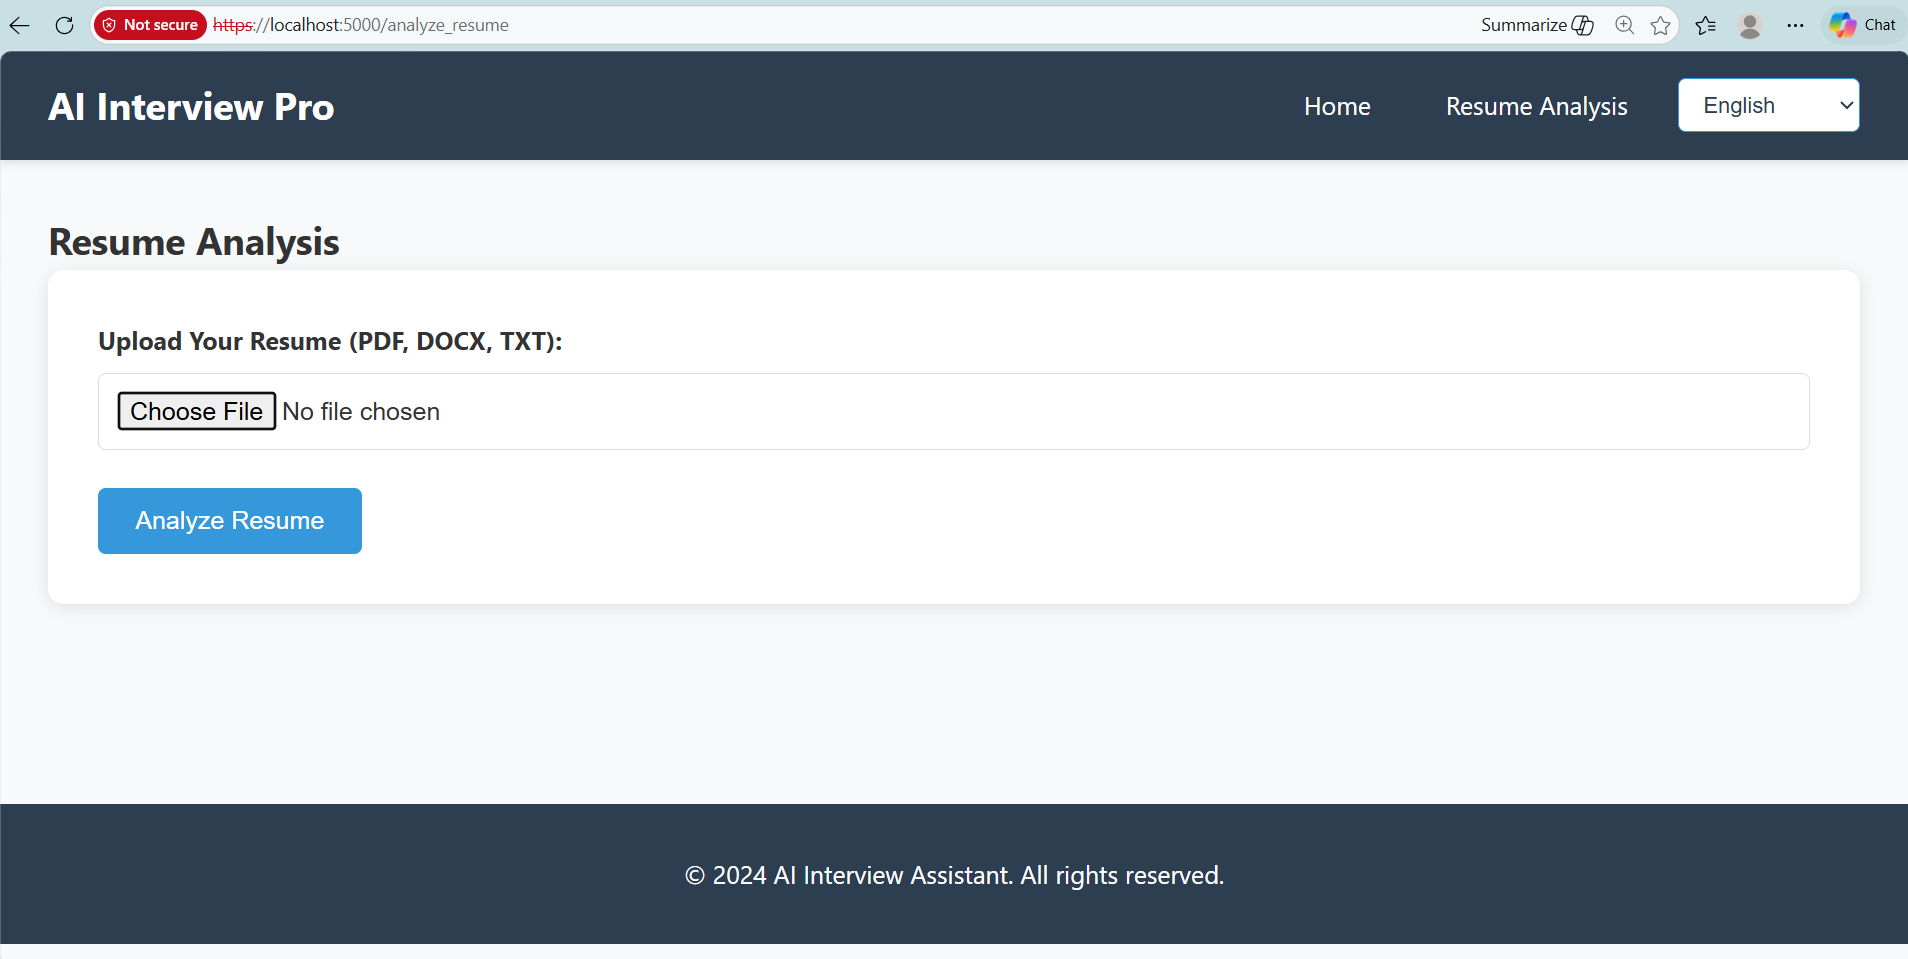
\includegraphics[width=0.99\textwidth]{op_2.png}}
\end{center}

\captionsetup{labelformat=empty}
\caption{Fig 8.1.2: Resume Analysis}
\label{fig:Device Initialization (Welcome Screen)}

\end{figure}

\vspace{10pt}

\begin{spacing}{1.5}
\noindent The resume analysis interface depicted in the figure 8.1.2 allows candidates to upload their professional documents for AI-driven evaluation. This page functions as a dedicated portal for collecting the candidate’s resume either prior to or independently of the interview process. When navigating to the “Resume Analysis” section, the system prompts the user to upload a document, supporting common file formats such as PDF, DOCX, and TXT. After selecting a file using the “Choose File” option and clicking the “Analyze Resume” button, the document is securely uploaded to the backend server for processing. The system then parses the file to extract key professional information, including skills, qualifications, and experience. Based on this analysis, an evaluation report is generated, and the extracted data can also be used to personalize and tailor the subsequent AI-driven interview questions according to the candidate’s background.\end{spacing}

\newpage

\begin{figure}[h]

\subsubsection*{8.1.3 : Resume Analysis Result Interface}

\vspace{10pt}

\begin{center}
\fbox{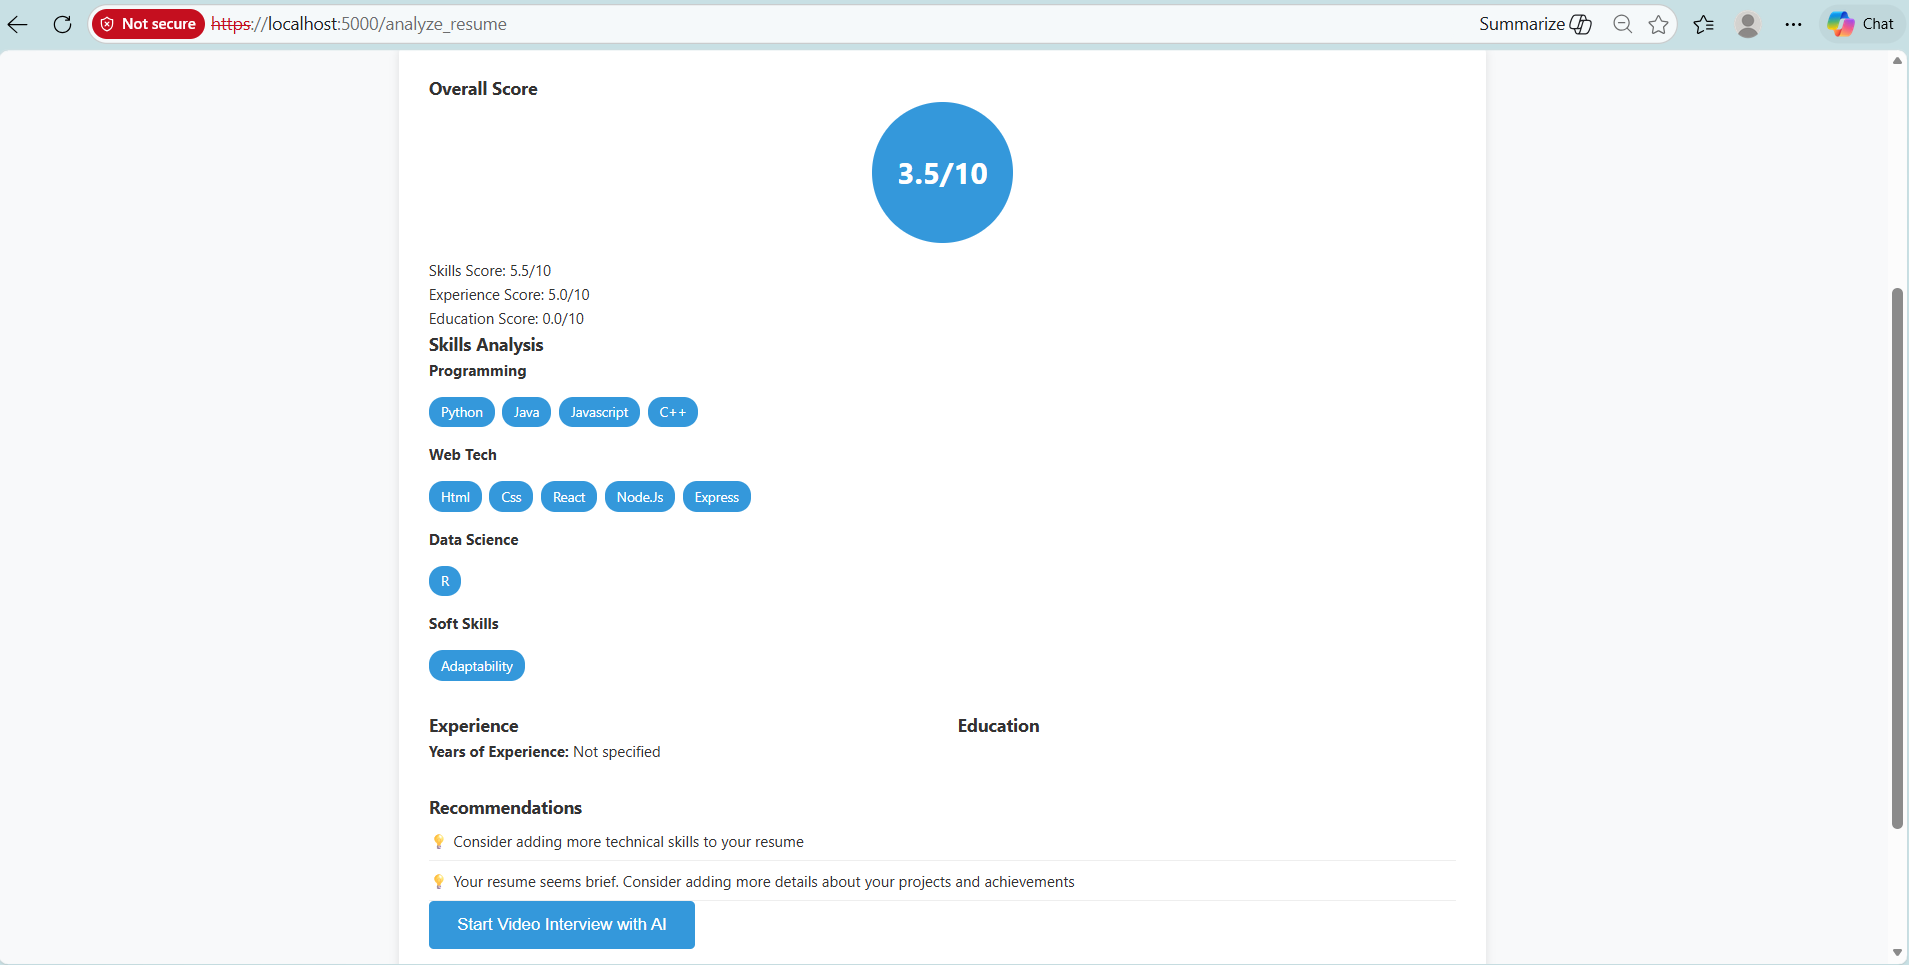
\includegraphics[width=0.99\textwidth]{op_3.png}}
\end{center}

\captionsetup{labelformat=empty}
\caption{Fig 8.1.3: Resume Analysis Result Interface}
\label{fig:Sensor Reading Display}

\end{figure}

\vspace{10pt}

\begin{spacing}{1.5}
\noindent The resume analysis results interface depicted in the figure 8.1.3 displays the detailed evaluation generated by the system after processing the candidate’s uploaded document, serving as a comprehensive feedback dashboard prior to the interview stage. Upon successful analysis, the system presents a prominent “Overall Score” at the top along with a detailed breakdown assessing key resume components such as Skills, Experience, and Education. The extracted information is organized into structured sections to provide meaningful insights; for instance, under the “Skills Analysis” section, identified competencies are grouped into relevant domains such as Programming, Web Technologies, Data Science, and Soft Skills using clear tag elements. The interface also highlights the availability or absence of information in the “Experience” and “Education” sections, enabling candidates to quickly identify areas where additional details may be required. Based on this analysis, the system generates actionable recommendations—such as adding more technical skills or elaborating on projects and achievements—to help improve the candidate’s professional profile. 
\end{spacing}

\newpage

\begin{figure}[h]

\subsubsection*{8.1.4 : Interview Interface}

\vspace{10pt}

\begin{center}
\fbox{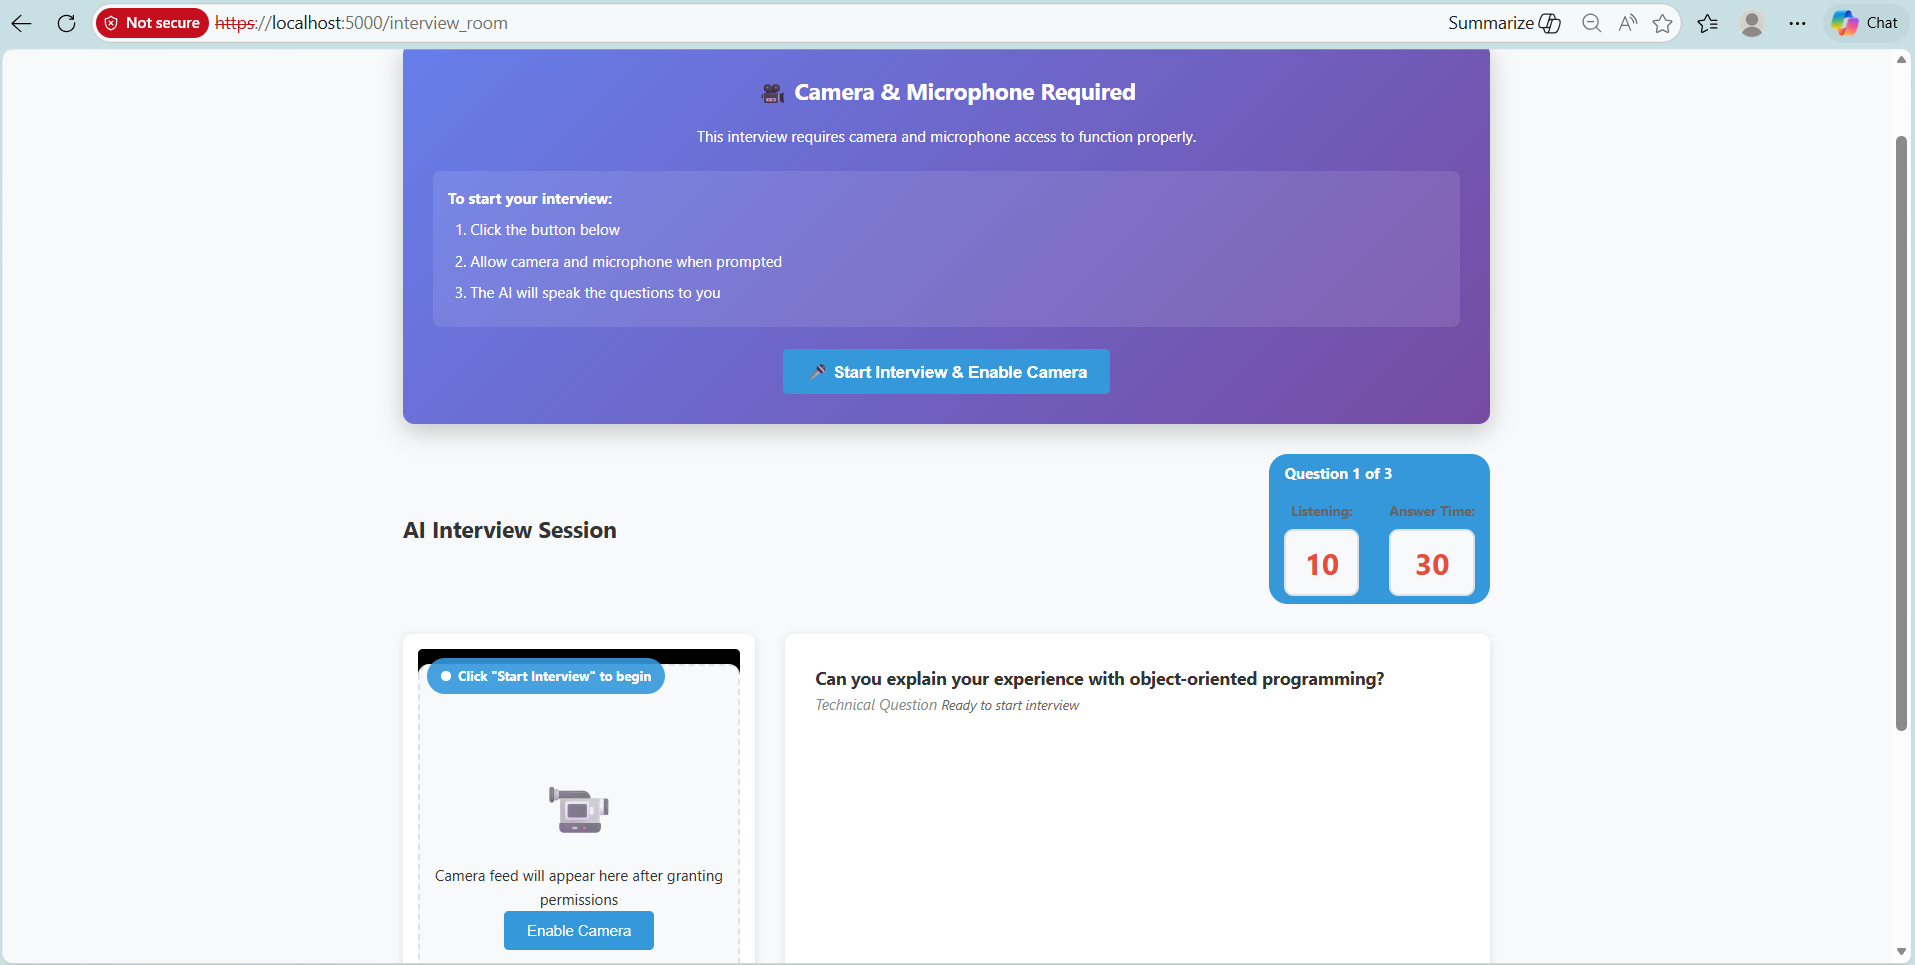
\includegraphics[width=0.99\textwidth]{op_4.png}}
\captionsetup{labelformat=empty}
\caption{Fig 8.1.4: Interview Interface}
\label{fig:Red Light Output}
\end{center}

\end{figure}

\vspace{10pt}

\begin{spacing}{1.5}
\noindent The AI interview session interface depicted in the figure 8.1.4 requires candidates to grant the necessary hardware permissions before commencing the live interactive evaluation and serves as the primary environment for conducting the video interview. Upon entering the interview room, a prominent notification informs the candidate that access to the camera and microphone is required, along with clear step-by-step instructions and a “Start Interview & Enable Camera” button to initiate the session. Once the candidate clicks the button and grants the required browser permissions, the system activates the local hardware and replaces the placeholder image with the candidate’s live camera feed. Simultaneously, the system displays the current AI-generated interview question—such as technical queries related to object-oriented programming—in the main area for the candidate to read and respond. Additionally, a tracking panel becomes active, presenting the overall session progress (for example, “Question 1 of 3”) and initiating real-time countdown timers that regulate the time allocated for listening to the prompt and recording the response, thereby ensuring a structured and time-bound interview experience.\end{spacing}

\newpage

\begin{figure}[h]

\subsubsection*{8.1.5 : Result Analysis}

\vspace{10pt}

\begin{center}
\fbox{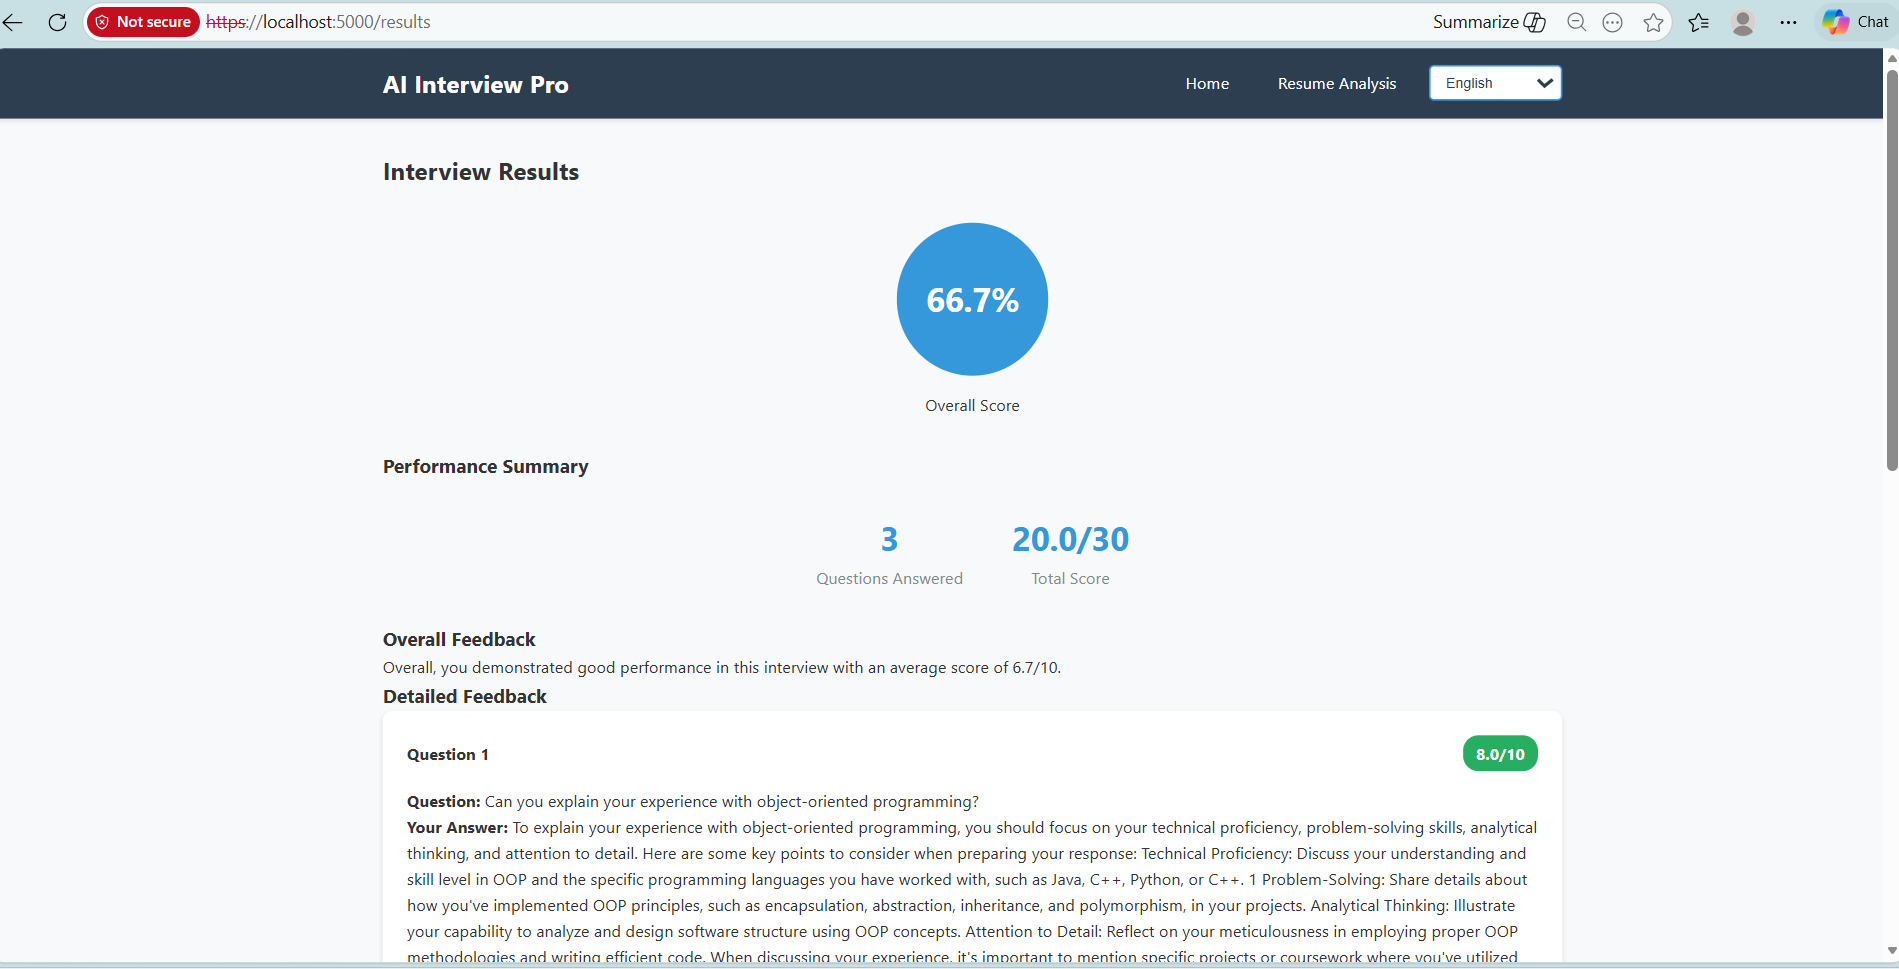
\includegraphics[width=0.99\textwidth]{op_5.png}}
\captionsetup{labelformat=empty}
\caption{Fig 8.1.5: Result Analysis}
\label{fig:Red Light Output}
\end{center}

\end{figure}

\vspace{10pt}

\begin{spacing}{1.5}
\noindent The interview results interface shown in Figure 8.1.5 presents a comprehensive evaluation of the candidate’s performance after completion of the AI-driven interview session. The system prominently displays the overall score as a percentage, providing an immediate summary of performance. A performance summary section indicates key metrics such as the number of questions answered and the total score obtained. Detailed feedback is provided for each question, including the original question, the candidate’s response, and constructive suggestions for improvement. The interface also highlights strengths and weaknesses by assigning individual scores to each question, enabling candidates to identify specific areas that require further preparation. Additionally, overall feedback summarizes the candidate’s performance across the session, and options such as starting a new interview or analyzing another resume allow the user to continue practicing seamlessly.

\end{document}